\hsection{Getting the Examples from this Book}%
\label{sec:gettingExamples}%
%
\begin{figure}%
\centering%
\subfloat[][%
How to download the examples.%
\label{fig:downloadExamples}%
]{\tightbox{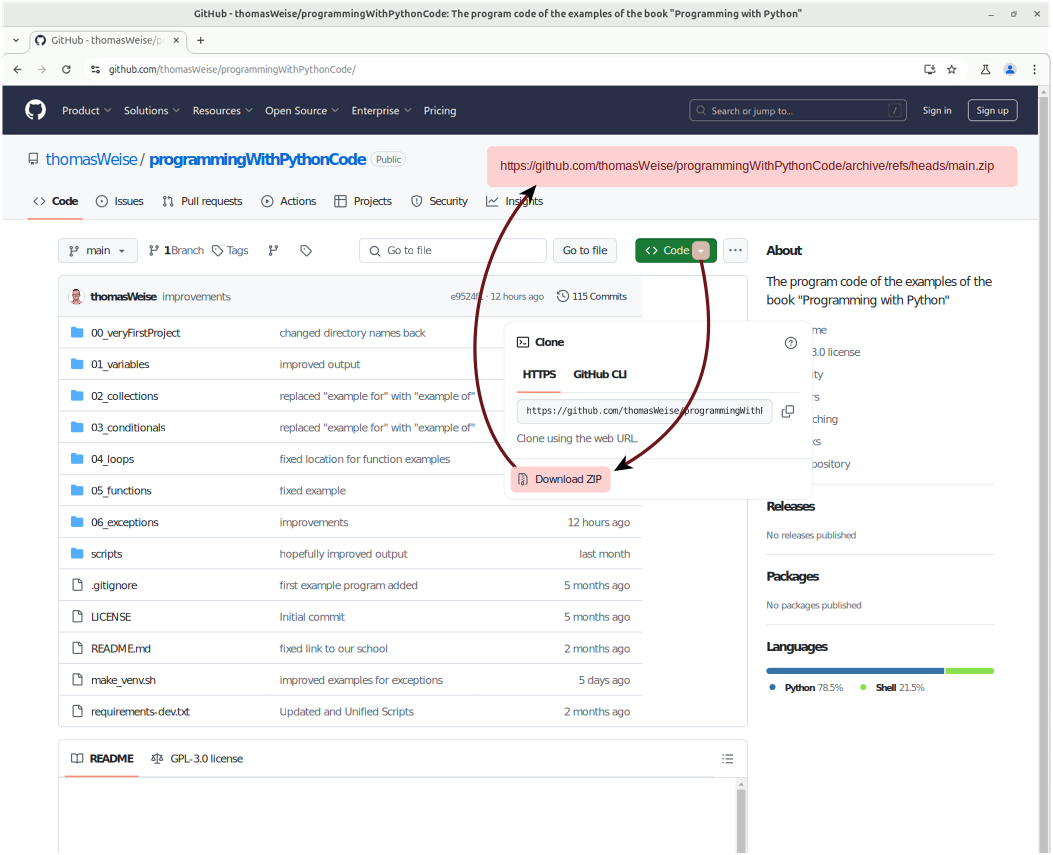
\includegraphics[width=0.8\linewidth,trim={0pt 1cm 0pt 0pt},clip]{\currentDir/downloadExamples}}}%
%
\floatRowSep%
%
\subfloat[][%
Visit the website \expandafter\url{\programmingWithPythonCodeRepo}. %
Then click on the downward facing triangle in the \menu{Code} button.%
\label{fig:downloadingExamples1website}%
]{\tightbox{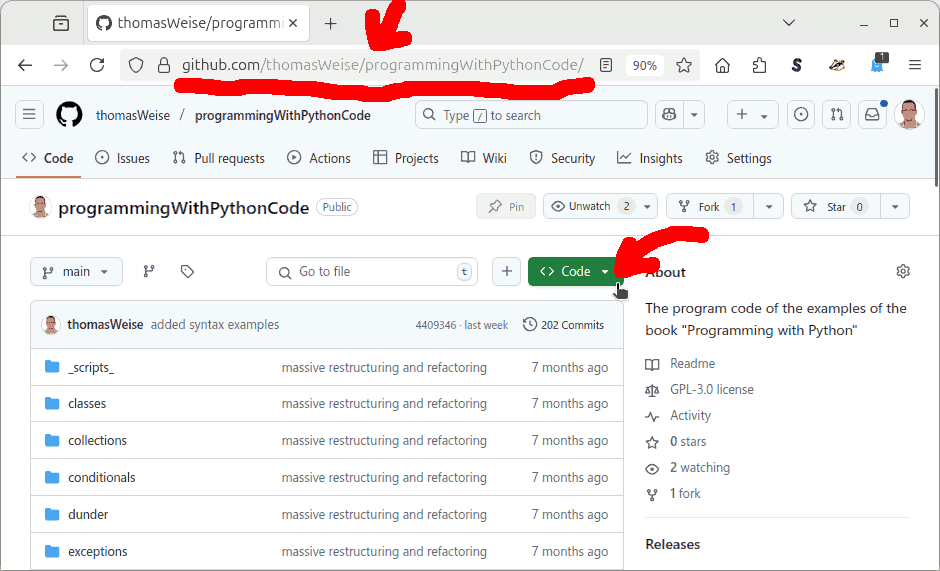
\includegraphics[width=0.45\linewidth]{\currentDir/downloadingExamples1website}}}%
%
\floatSep%
%
\subfloat[][%
In the popup menu that appears, click \menu{Download ZIP}.%
\label{fig:downloadingExamples2download}%
]{\tightbox{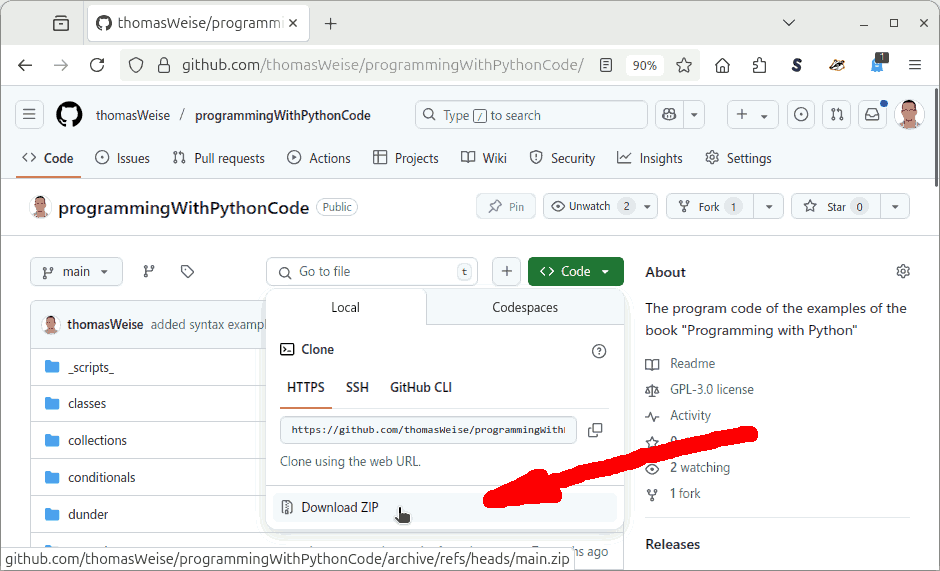
\includegraphics[width=0.45\linewidth]{\currentDir/downloadingExamples2download}}}%
%
\floatRowSep%
%
\subfloat[][%
The \texttt{zip}~archive is downloaded.%
\label{fig:downloadingExamples3downloaded}%
]{\tightbox{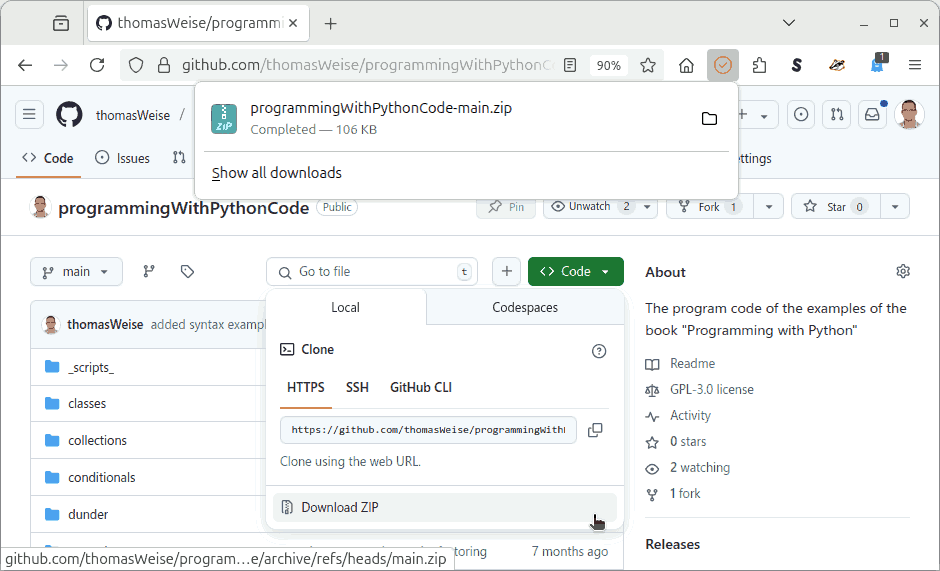
\includegraphics[width=0.45\linewidth]{\currentDir/downloadingExamples3downloaded}}}%
%
\floatSep%
%
\subfloat[][%
We click on it to open it.%
\label{fig:downloadingExamples4open}%
]{\tightbox{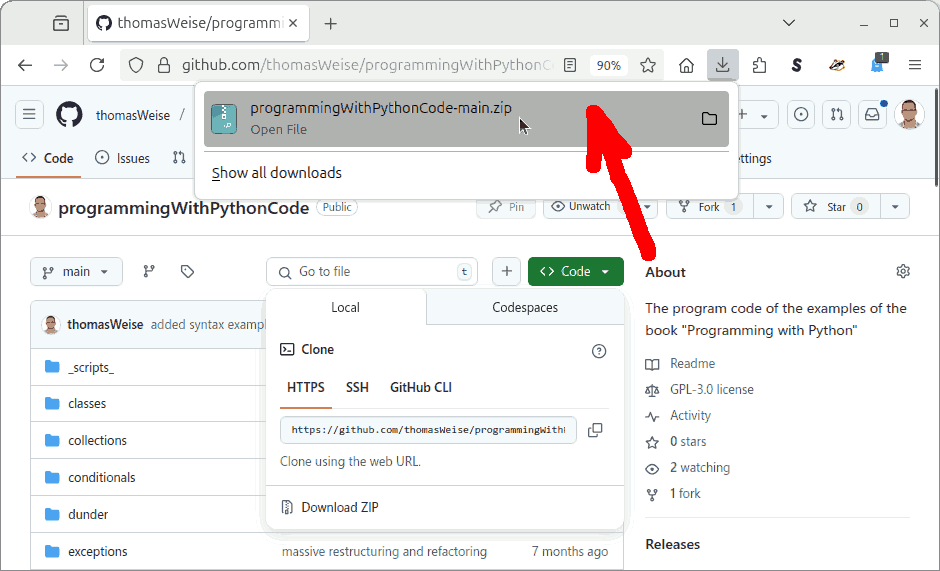
\includegraphics[width=0.45\linewidth]{\currentDir/downloadingExamples4open}}}%
%
\caption{Downloading all the example source codes as a single \texttt{zip}~archive from \expandafter\url{\programmingWithPythonCodeRepo}.}%
\label{fig:downloadExamplesA}%
\end{figure}%
%
\begin{figure}%
\ContinuedFloat%
\centering%
%
\subfloat[][%
The archive opens and shows us the root folder of the archive. %
We open this folder.%
\label{fig:downloadingExamples5zipOpened}%
]{\tightbox{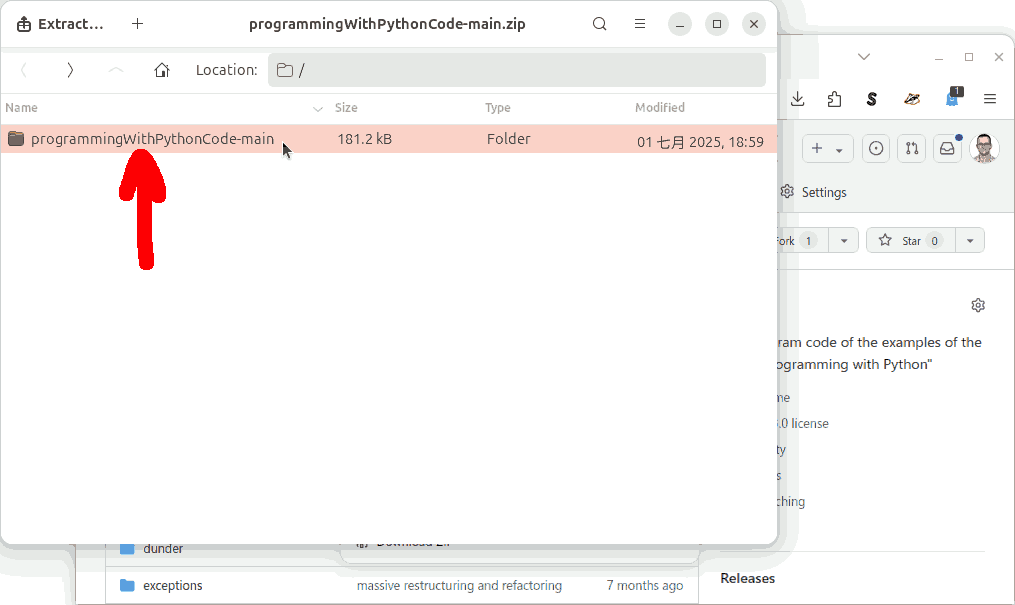
\includegraphics[width=0.45\linewidth]{\currentDir/downloadingExamples5zipOpened}}}%
%
\floatSep%
%
\subfloat[][%
Now you can see all the example folders. %
The folder \bashil{veryFirstProject} includes the Hello-World example we just discussed.%
\label{fig:downloadingExamples6veryFirstProject}%
]{\tightbox{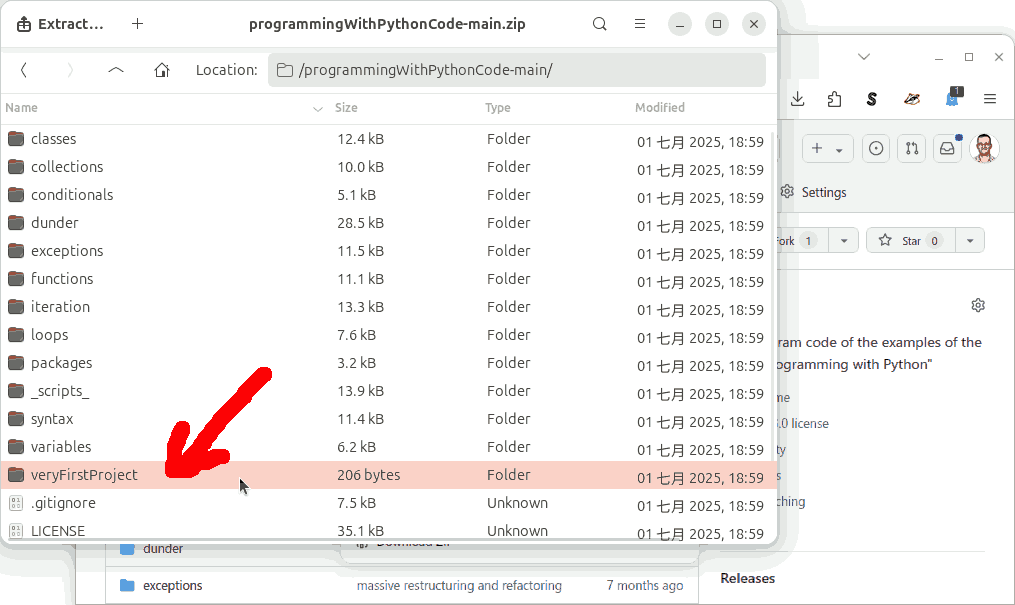
\includegraphics[width=0.45\linewidth]{\currentDir/downloadingExamples6veryFirstProject}}}%
%
\caption{Downloading all the example source codes as a single \texttt{zip}~archive from \expandafter\url{\programmingWithPythonCodeRepo}~(Continued).}%
\label{fig:downloadExamplesB}%
\end{figure}%
%
\begin{figure}%
\centering%
%
\subfloat[][%
Click \menu{Clone Repository} in the \pycharm\ welcome screen.%
\label{fig:clone01welcomeToPycharm}%
]{\tightbox{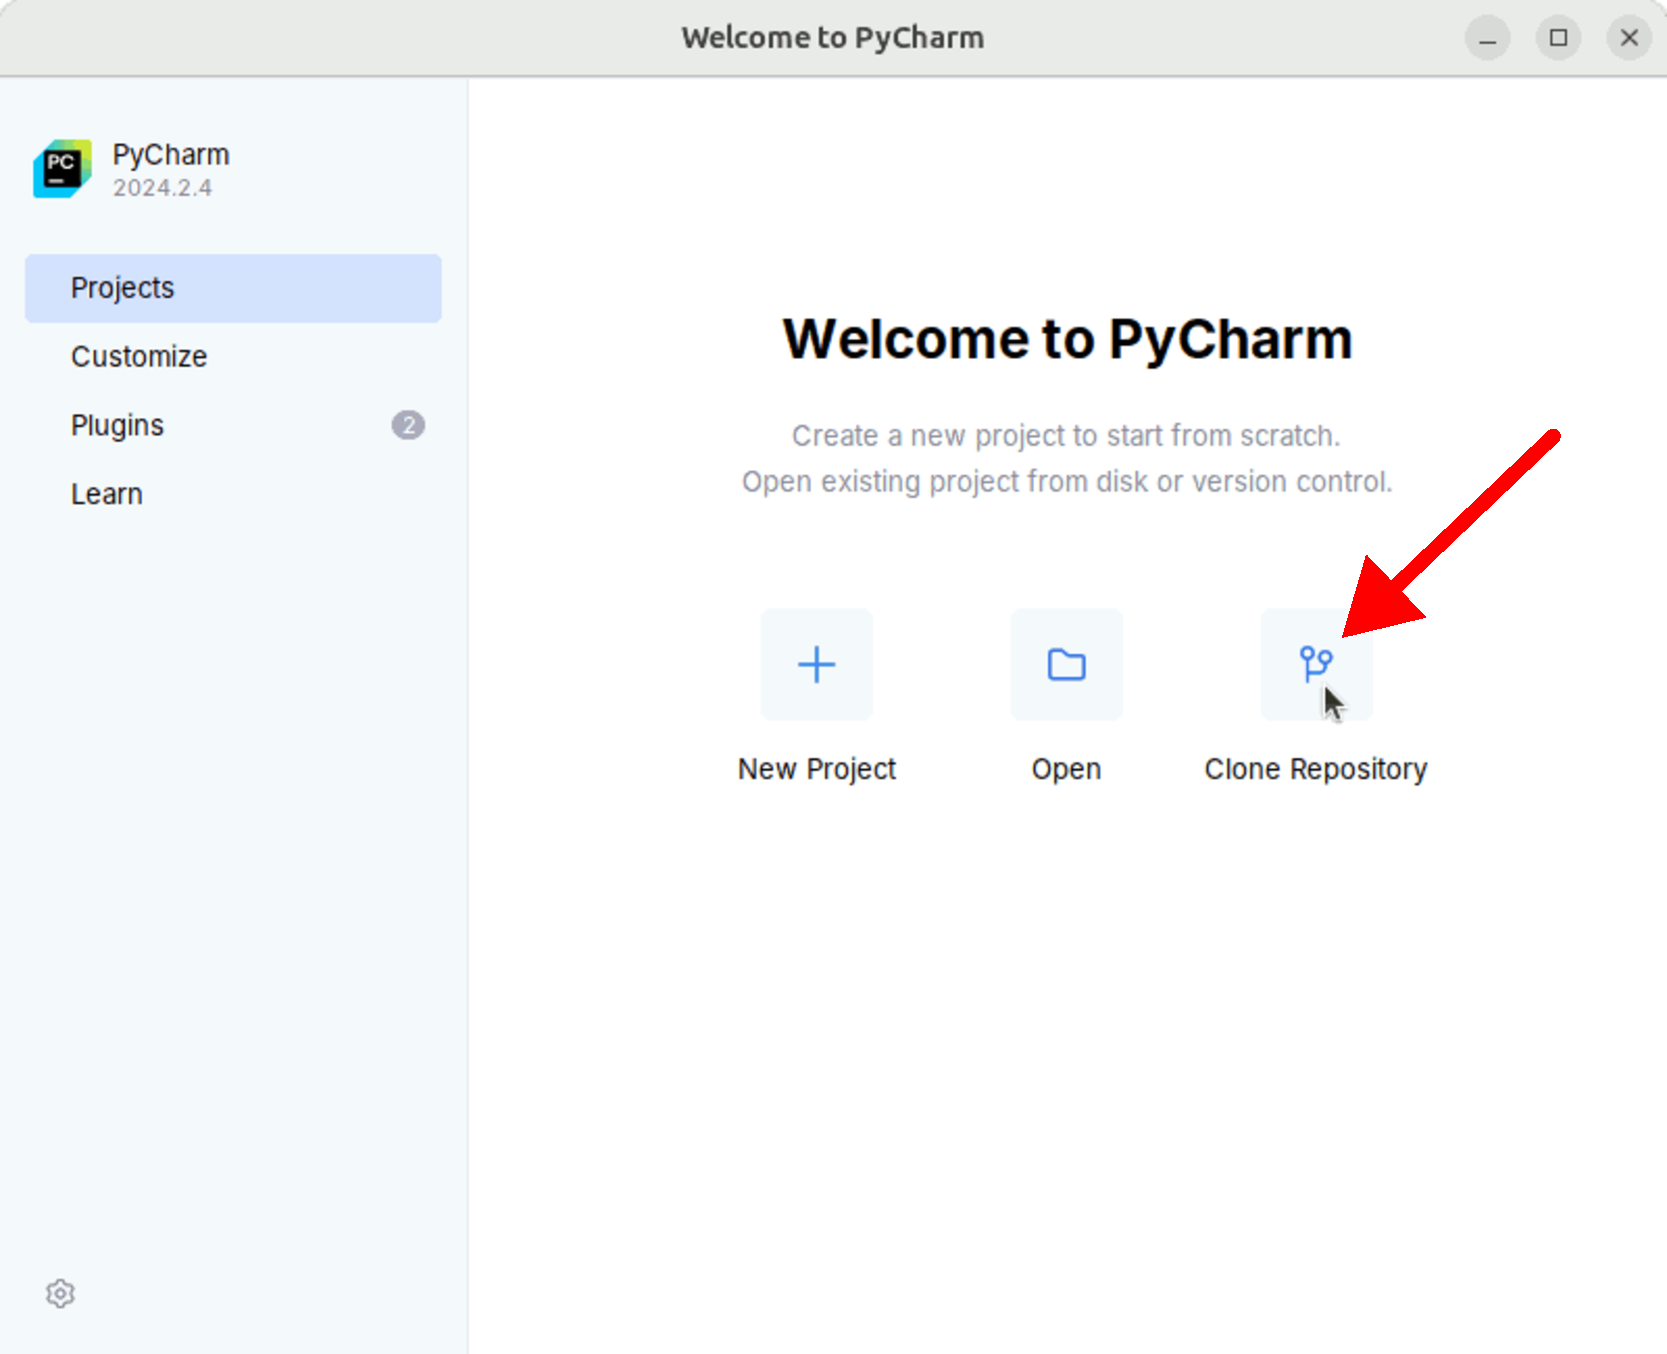
\includegraphics[width=0.45\linewidth]{\currentDir/clone01welcomeToPycharm.pdf}}}%
%
\floatSep%
%
\subfloat[][%
Selecting \menu{URL:} \expandafter\url{\programmingWithPythonCodeRepo} and a reasonable destination \menu{Directory:} in the next dialog, then click \menu{Clone}.%
\label{fig:clone02selectRepoAndDestination}%
]{\tightbox{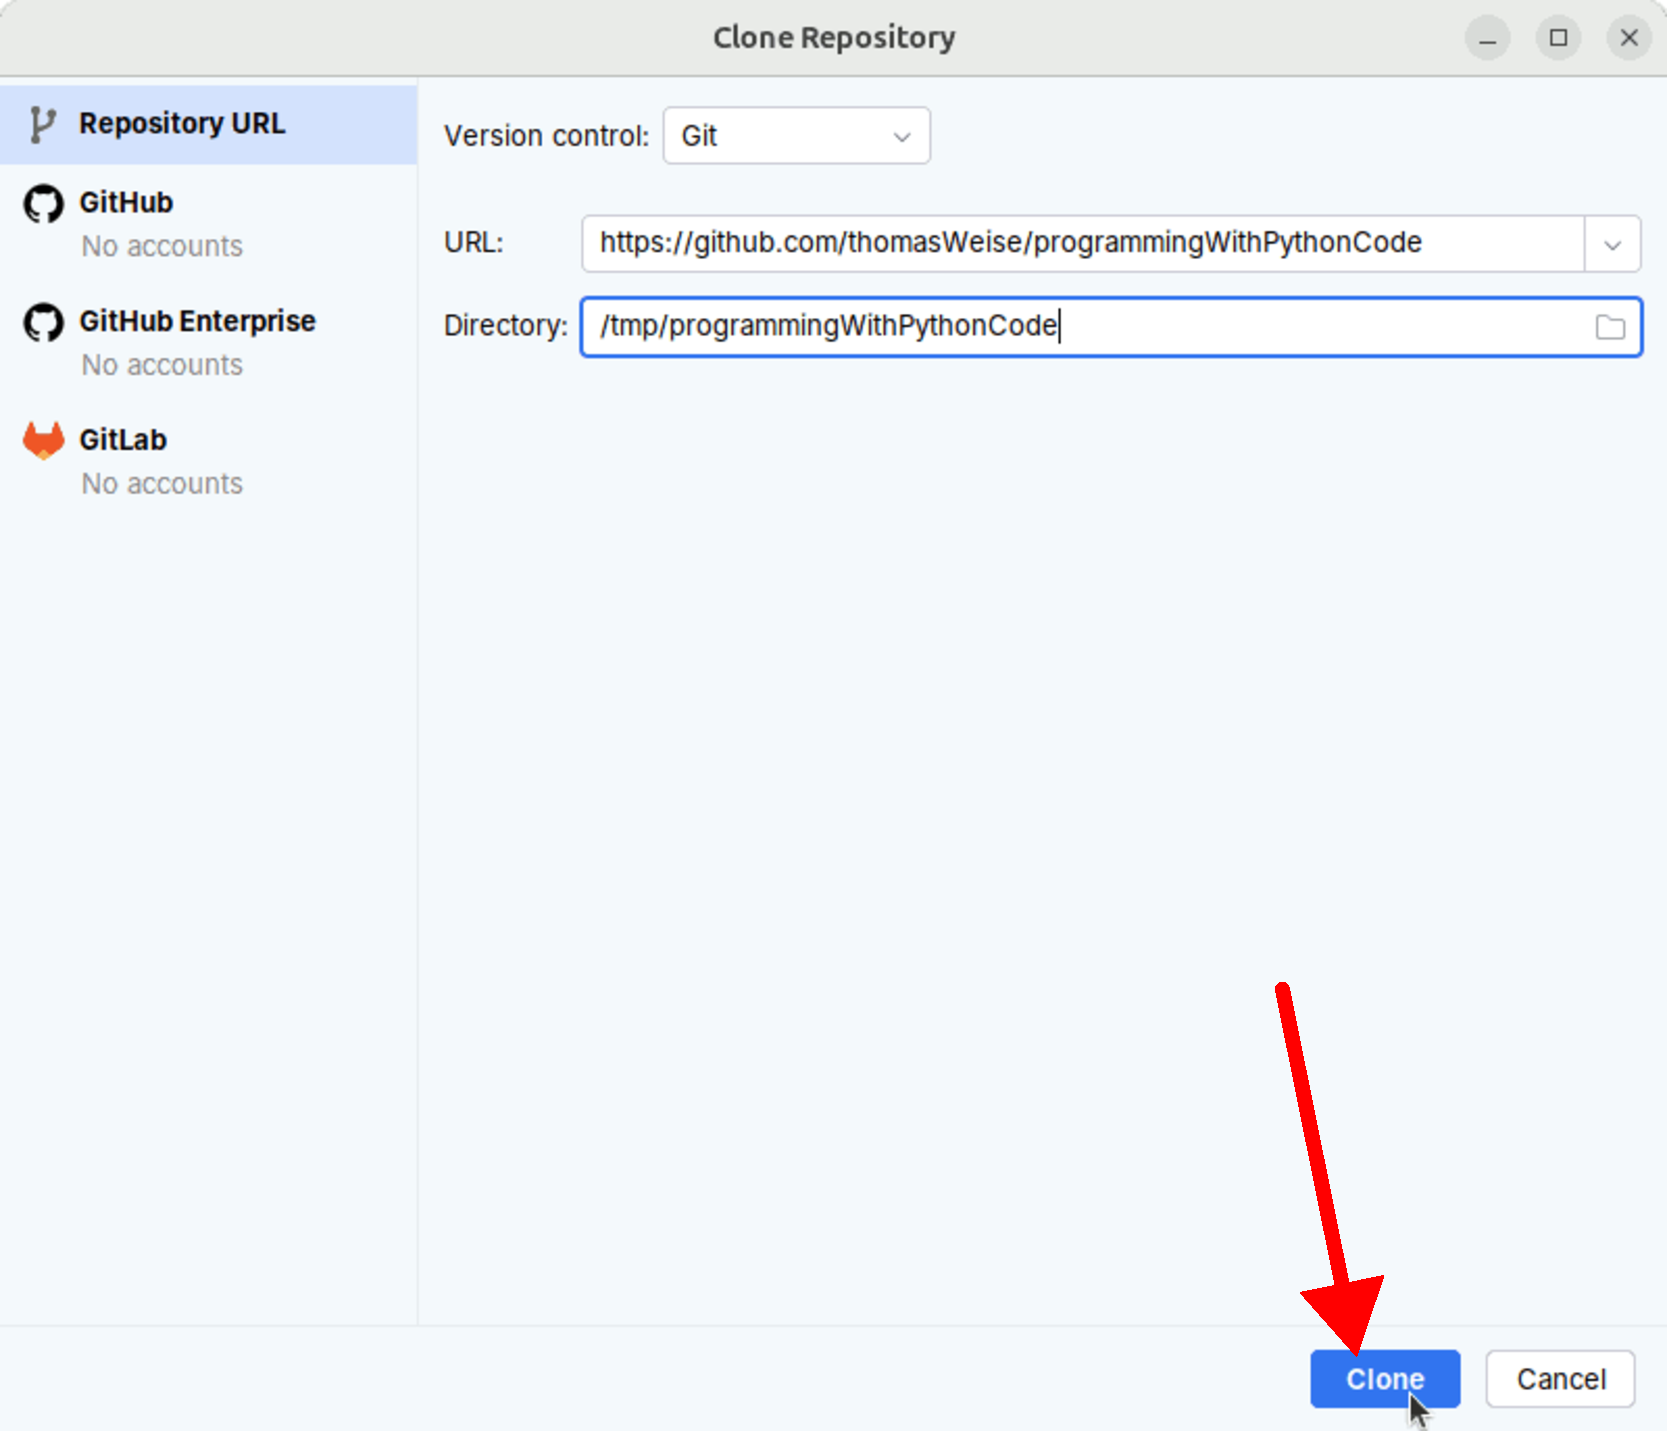
\includegraphics[width=0.45\linewidth]{\currentDir/clone02selectRepoAndDestination.pdf}}}%
%
\floatRowSep%
%
\subfloat[][%
Wait while \pycharm\ is cloning (downloading) the repository.%
\label{fig:clone03cloning}%
]{\tightbox{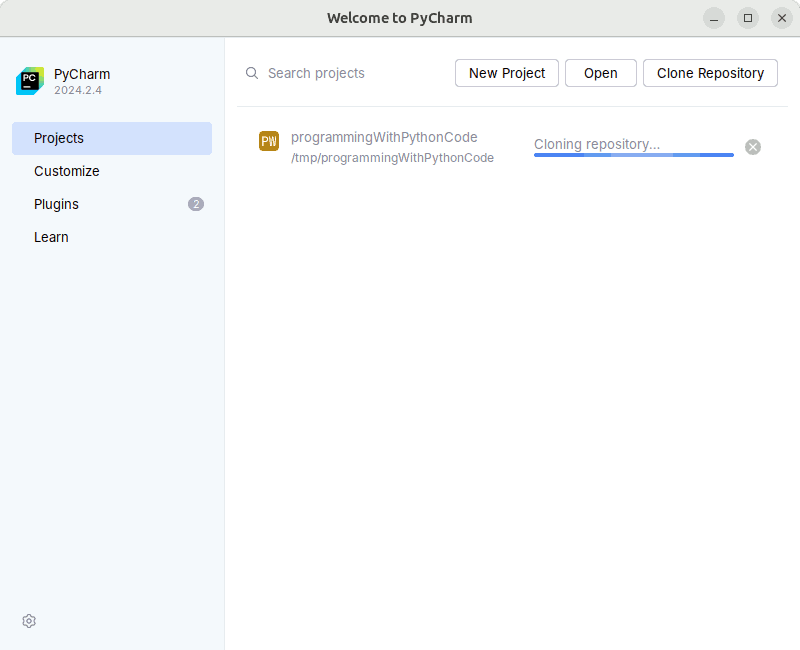
\includegraphics[width=0.45\linewidth]{\currentDir/clone03cloning}}}%
%
\floatSep%
%
\subfloat[][%
If asked, click \menu{Trust Project} after confirming that you indeed downloaded the right code and if you trust our code.%
\label{fig:clone04trustProject}%
]{\tightbox{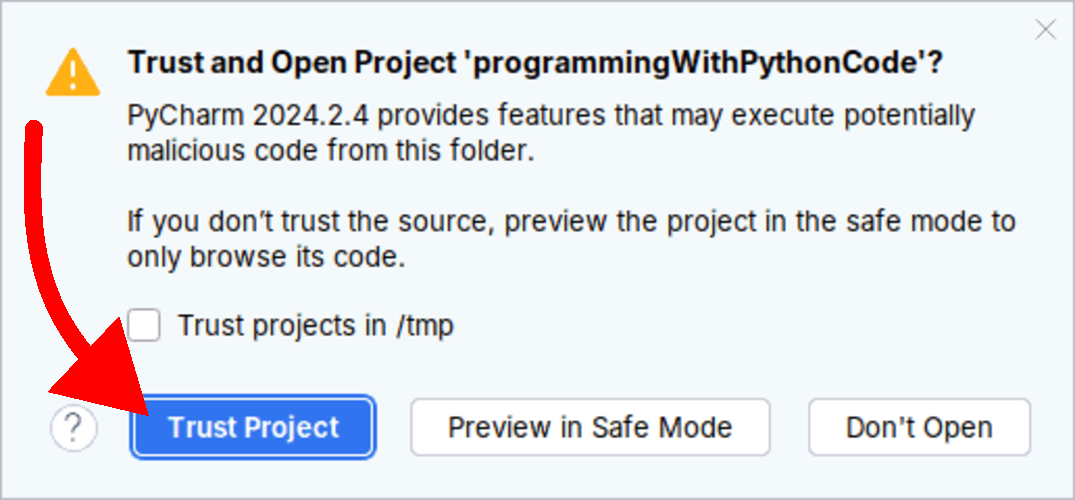
\includegraphics[width=0.45\linewidth]{\currentDir/clone04trustProject.pdf}}}%
%
\floatRowSep%
%
\subfloat[][%
The project with all the examples from this book is now downloaded and can be accessed in \pycharm.%
\label{fig:clone05finished}%
]{\tightbox{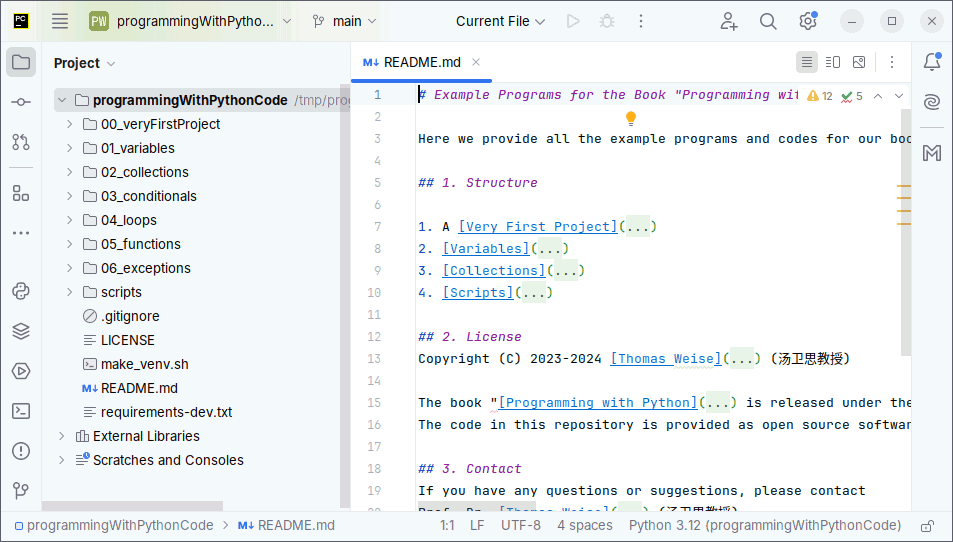
\includegraphics[width=0.6\linewidth]{\currentDir/clone05finished}}}%
%
\caption{Using \pycharm\ to clone (download) and import all the examples from this book.}%
\label{fig:cloningExamples}%
\end{figure}%
%
This book comes with a lot of examples programs written in \python.
While our first explorations of the simple data types will mainly use the \python\ console, we will later almost exclusively write programs in \python\ files.
Every single one of them is available in the \pgls{git} repository \texttt{\programmingWithPythonCodeRepoName}.
You can directly access this repository at \pgls{github} under \expandafter\url{\programmingWithPythonCodeRepo}.%
%
\begin{sloppypar}%
On the website, you can directly download all the examples as illustrated in \cref{fig:downloadExamples}.
First, you would click on the little downward facing triangle in the button \menu{Code} as shown in~\cref{fig:downloadingExamples1website}.
This will open a small dialog \menu{Clone} in which you can click on the \menu{Download ZIP} button~(see \cref{fig:downloadingExamples2download}).
This, in turn, enters the \pgls{URL}~\expandafter\url{\programmingWithPythonCodeRepo/archive/refs/heads/main.zip} into your browser's download queue.
\end{sloppypar}%
%
The download will eventually finish, as shown in \cref{fig:downloadingExamples3downloaded}, at which point you can open the downloaded \texttt{zip}~archive by clicking on it as sketched in \cref{fig:downloadingExamples4open}.
A \texttt{zip}~archive is a single file that can contain other files and folders and can be opened by the standard file managers both on \ubuntu\ and \microsoftWindows.
Once downloaded, the archive contains all the examples that we use in our book.
Its root folder is named similarly to the repository~(see \cref{fig:downloadingExamples5zipOpened}).
Inside this folder, you can find all the folders with examples, including the example \bashil{veryFirstProject} we just discussed in the previous section, as shown in~\cref{fig:downloadingExamples6veryFirstProject}.

Alternatively to downloading a \texttt{zip}~archive with the examples from this book, you can also directly create a new project in \pycharm\ by cloning (basically, downloading) the repository as illustrated in \cref{fig:cloningExamples}.
You see, our examples are all located in a so-called \git\ repository~\cite{S2023LG,T2024BGAGVCPMATFTND}.
\git\ is a \glsreset{VCS}\pgls{VCS}~\cite{S2023LG,T2024BGAGVCPMATFTND}, i.e., a version management system for software development.
With such a system, we can iteratively work on our code and commit changes to the code base.
The \pgls{VCS} remembers the history of our projects and allows us to share and collaboratively work on the code.
Well, we will not collaboratively work on this code with each other, because the code represents artificial examples for a course.
But \git\ is a very well-known and widely-used \pgls{VCS}, so at least getting familiar with it does not hurt.
Our examples are hosted in a \git\ repository on \github~\cite{PRGWSUdVLFTEKPKFBV2016TSRFTAOGAG,T2024BGAGVCPMATFTND}.
And you can clone it just as well instead of just downloading it.

\begin{sloppypar}%
In the \pycharm\ welcome screen, you click \menu{Clone Repository} as shown in \cref{fig:clone01welcomeToPycharm}.
In the next dialog, you have to select a source \menu{URL:}, which will be \expandafter\url{\programmingWithPythonCodeRepo}.
You also need to choose a \menu{Directory:} where the new project should be located.
All the contents of the examples repository will be downloaded into this directory as well.
In \cref{fig:clone02selectRepoAndDestination}, I selected \textil{/tmp/programmingWithPythonCode}, i.e., a directory on my partition for temporary files.
This directory will be cleared at every system boot, so you would certainly choose a more reasonable destination.
After clicking \menu{Clone}, the downloading will begin, as sketched in \cref{fig:clone03cloning}.%
\end{sloppypar}%
%
Once the repository has been downloaded, \pycharm\ may ask you whether you trust this project.
After making sure that you indeed downloaded the examples for this book (and if you deem this code trustworthy), you can click \menu{Trust Project}, as \cref{fig:clone04trustProject}.
Finally, as \cref{fig:clone05finished} shows, you can now see and play with and run all the examples in \pycharm.
A more comprehensive discussion on how to clone repositories is given in \cref{sec:gitClone}.%
%
\FloatBarrier%
\endhsection%
%
